\section{Implementation and evaluation}

\subsection{Environments with Evolving Objectives}
We begin by describing the multi-objective environments that we evaluate our framework on. Despite their practical relevance, environments with multiple evolving objectives have received little attention in the multi-objective RL literature.

\textbf{Dynamic Targets.}\quad We implement a simple but challenging gridworld environment called Dynamic Targets which consists of an \(n \times n\) grid with \(m\) targets that are moving at a small rate and stochastically change directions. Each target stays alive for a certain number of timesteps before which the agent has to reach it. Once the target expires or the agent reaches it, another new target immediately respawns at a random position in the grid. The metric the agent has to maximize is the difference between the number of targets reached and the number of targets that expired. This flexible environment also allows us to introduce more targets at deployment time. \todo{Reference image for benchmark}

\textbf{Atari Assault.}\quad We also test our method on the Atari game Assault. Here, we control a missile and shoot alien ships that move. Even though this is not a multi-objective environment, we decompose it so that we can treat each alien ship as a different objective. Since these alien ships move around and there are a variable number of ships at any point of time, it is a perfect testbed for our modular approach. We check whether we can synthesize interpretable policies that split control of the missile to target different ships. However, as the standard Atari games from the Arcade Learning Environment \citep{bellemare13arcade} either use image or raw RAM observations, we cannot decompose the game score and design rewards for the multiple policies. Instead, we turn to the Object-Centric Atari environments \citep{delfosse2023ocatari} which exposes object positions and states by decoding RAM states. This permits us to design decomposed observations and rewards for each policy to pursue and shoot the alien ships. \todo{Add image of Assault.}

\subsection{Implementation and Training}
\citet{yu2022mappo} demonstrate how we can train policies concurrently in multi-agent settings using proximal policy optimization (PPO; \cite{schulman2017ppo}). We follow their recipe and train all the policies with PPO. We also share the actor and critic network parameters across all the policies since the objectives in our environments share the same characteristics.

Additionally, in the Dynamic Targets environments, we employ an attention pooling architecture to encode information about all the targets. This allows the policies to generalize to arbitrary number of targets at deployment time.

\subsection{Baselines}

\subsection{Experimental results}

\subsection{Implementation}
Talk about:
\begin{enumerate}
    \item different bidding mechanisms
    \item choice of penalty factor
    \item action window (remarking that we could additionally allow agents to choose length of action window)
    \item use with off-the-shelf RL algorithms
\end{enumerate}

\subsection{Environments}

\subsubsection{MovingTargetsGridworld}
Important to mention that we want to maximize \(\min(\text{targets reached})\).

\subsubsection{Atari Assault}

\subsection{Baselines}
\begin{enumerate}
    \item Weighted sum of rewards with standard RL algorithms
    \item Deep W learning implemented on top of DQN
\end{enumerate}

\subsection{Performance comparison with baselines}
Include plots of training steps vs performance of our algorithms vs baselines on both environments

\begin{figure}[h]
    \centering
    \begin{subfigure}{0.48\textwidth}
        \centering
        
\includegraphics[width=\textwidth]{img/gridworld_bidding_mechanisms_learning_curves.png}
        \caption{MovingTargetsGridworld. [Placeholder: describe convergence behavior, relative performance of mechanisms, and any notable differences in sample efficiency.]}
        \label{fig:gridworld-bidding-mechanisms}
    \end{subfigure}
    \hfill
    \begin{subfigure}{0.48\textwidth}
        \centering
        
\includegraphics[width=\textwidth]{img/assault_bidding_mechanisms_learning_curves.png}
        \caption{Atari Assault. [Placeholder: describe convergence behavior, relative performance of mechanisms, and any notable differences in sample efficiency.]}
        \label{fig:assault-bidding-mechanisms}
    \end{subfigure}
    \caption{Learning curves for different bidding mechanisms across both environments.}
    \label{fig:bidding-mechanisms}
\end{figure}

\begin{table}
  \centering
  \caption{Performance (mean with 95\% CI) averaged over the last 5 evaluation checkpoints.}
  \begin{tabular}{lll}
    \hline
    {\bf Algorithm} & {\bf Gridworld (Min Targets Reached)} & {\bf Assault (Score)}
    \\ \hline
    All-Pay & $6.05$ {\small\textcolor{gray}{$[5.74,\ 6.36]$}} & $634.80$ {\small\textcolor{gray}{$[591.14,\ 678.46]$}} \\
    Winner-Pays & $4.07$ {\small\textcolor{gray}{$[3.78,\ 4.36]$}} & $578.04$ {\small\textcolor{gray}{$[521.02,\ 635.06]$}} \\
    Winner-Pays (Others Rewarded) & $4.20$ {\small\textcolor{gray}{$[3.92,\ 4.48]$}} & $662.60$ {\small\textcolor{gray}{$[619.09,\ 706.11]$}} \\
    Single-Agent & $2.31$ {\small\textcolor{gray}{$[2.08,\ 2.54]$}} & $384.72$ {\small\textcolor{gray}{$[343.09,\ 426.35]$}} \\
    DWN & $0.98$ {\small\textcolor{gray}{$[0.75,\ 1.21]$}} & $256.20$ {\small\textcolor{gray}{$[205.12,\ 307.28]$}} \\
    \hline
  \end{tabular}
  \label{tab:bidding_comparison}
\end{table}

\subsection{Interpretability}
Include plots of distribution of control steps amongst agents, table of average, median, max, min of bids of agents

\subsection{Modularity}
Plots of performance in gridworld with increasing number of objectives

\subsection{Ablations}
Impact of max bid, penalty factor

\begin{figure}[h]
    \centering
    \begin{subfigure}[b]{0.3\textwidth}
        \centering
        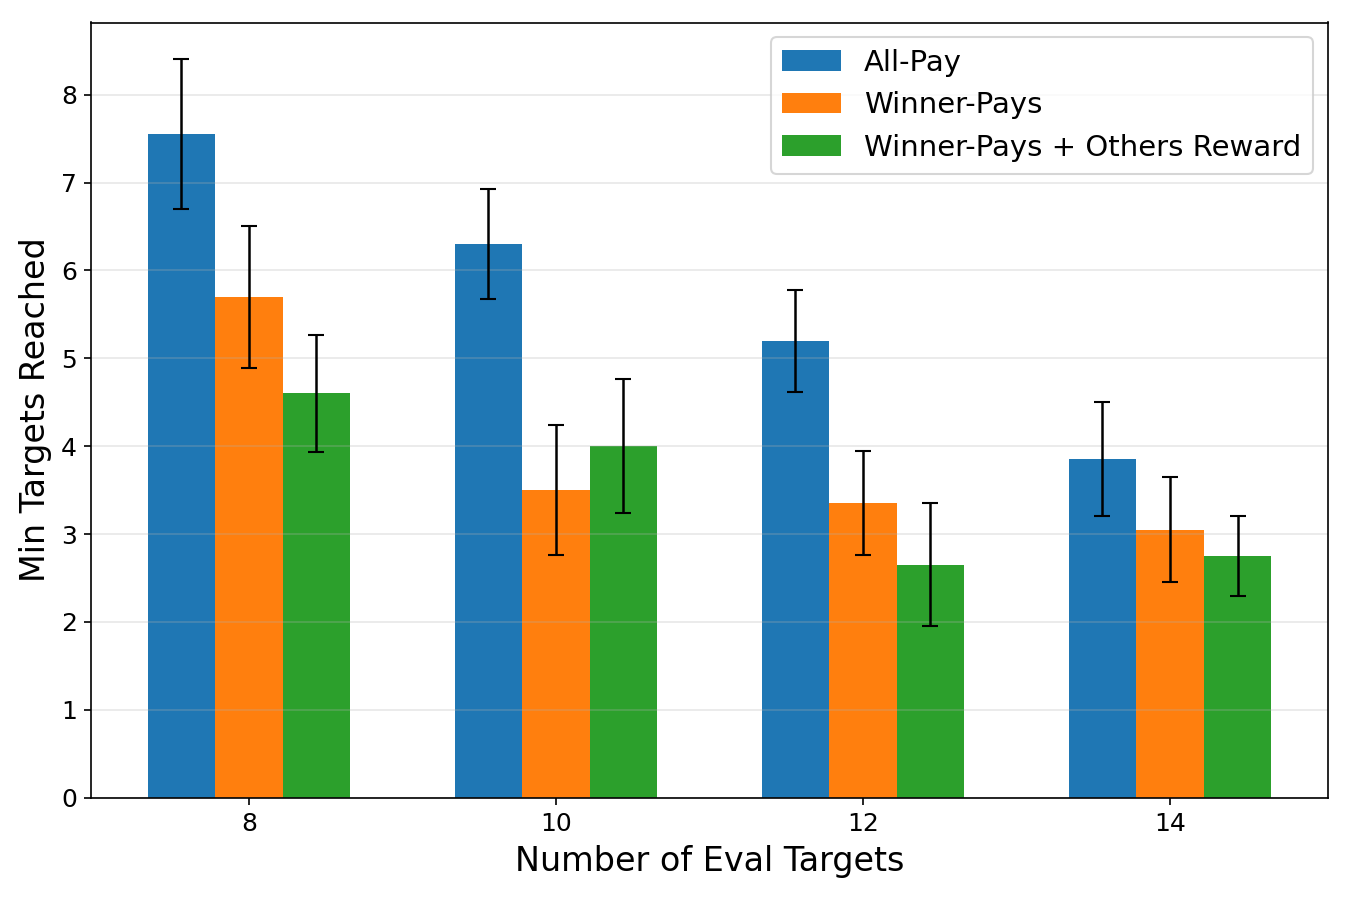
\includegraphics[width=\textwidth]{img/bidding_mechanism_scaling.png}
        \caption{Bidding mechanism scaling. [Placeholder description.]}
        \label{fig:bidding-mechanism-scaling}
    \end{subfigure}
    \hfill
    \begin{subfigure}[b]{0.3\textwidth}
        \centering
        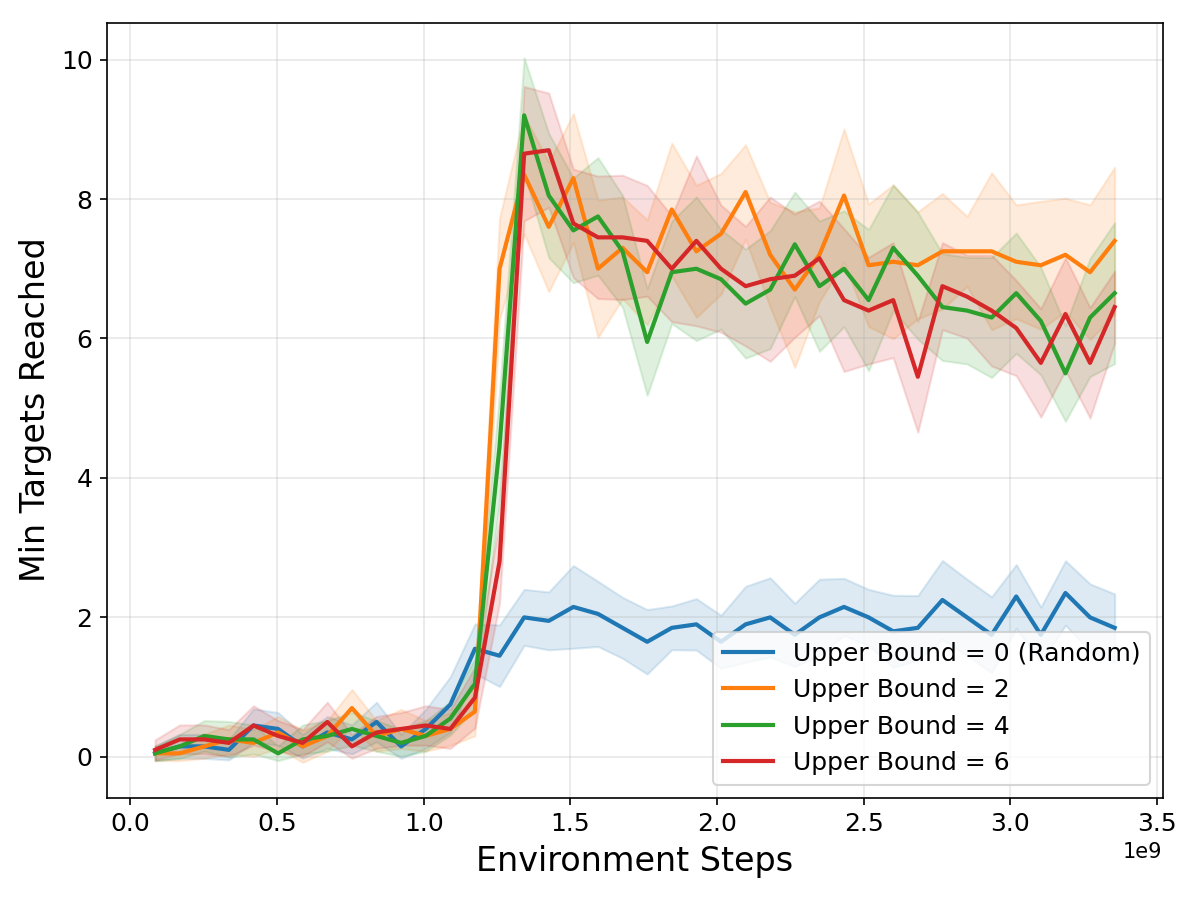
\includegraphics[width=\textwidth]{img/gridworld_bid_upper_bound_learning_curves.png}
        \caption{Bid upper bound. [Placeholder description.]}
        \label{fig:gridworld-bid-upper-bound}
    \end{subfigure}
    \hfill
    \begin{subfigure}[b]{0.3\textwidth}
        \centering
        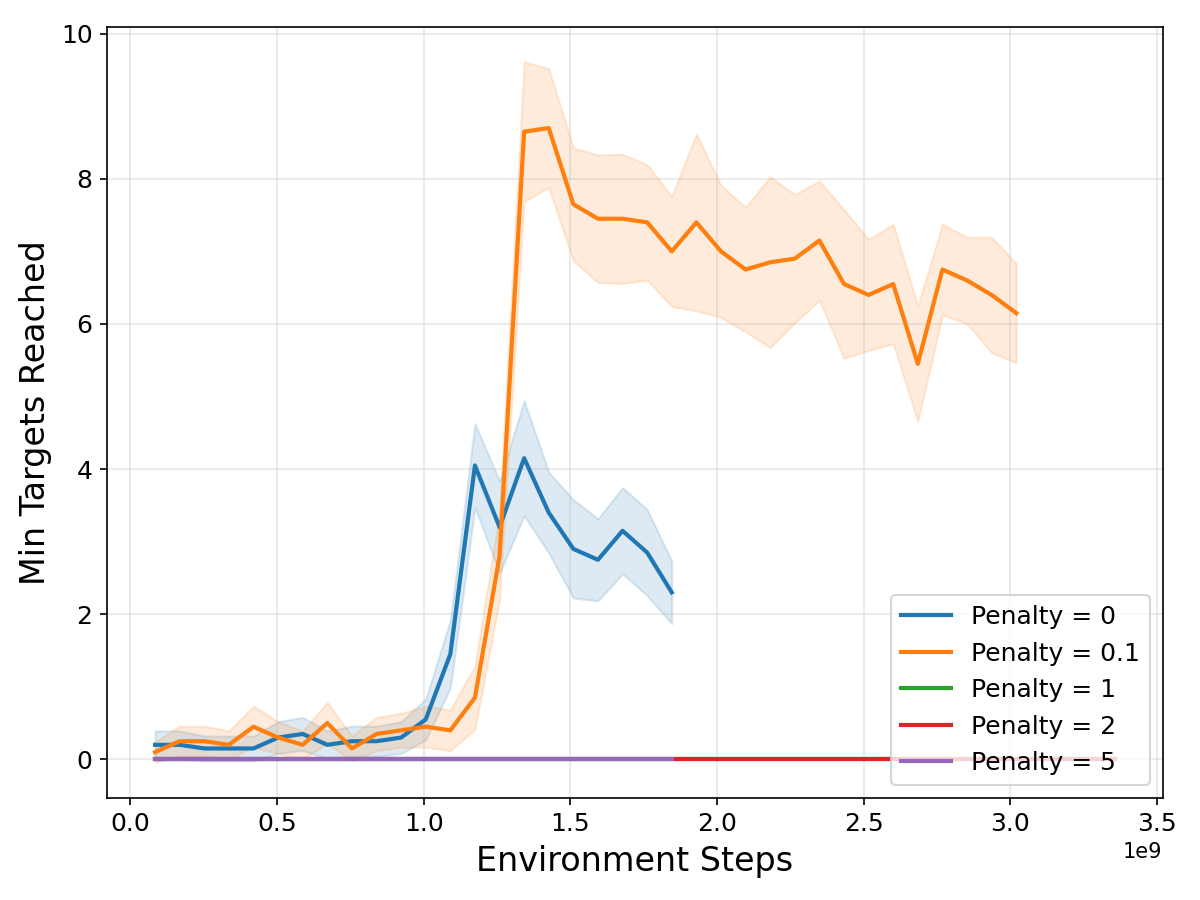
\includegraphics[width=\textwidth]{img/gridworld_bid_penalty_learning_curves.png}
        \caption{Bid penalty. [Placeholder description.]}
        \label{fig:gridworld-bid-penalty}
    \end{subfigure}
    \caption{Ablation studies on the MovingTargetsGridworld environment.}
    \label{fig:ablations}
\end{figure}

\begin{figure}[h]
    \centering
    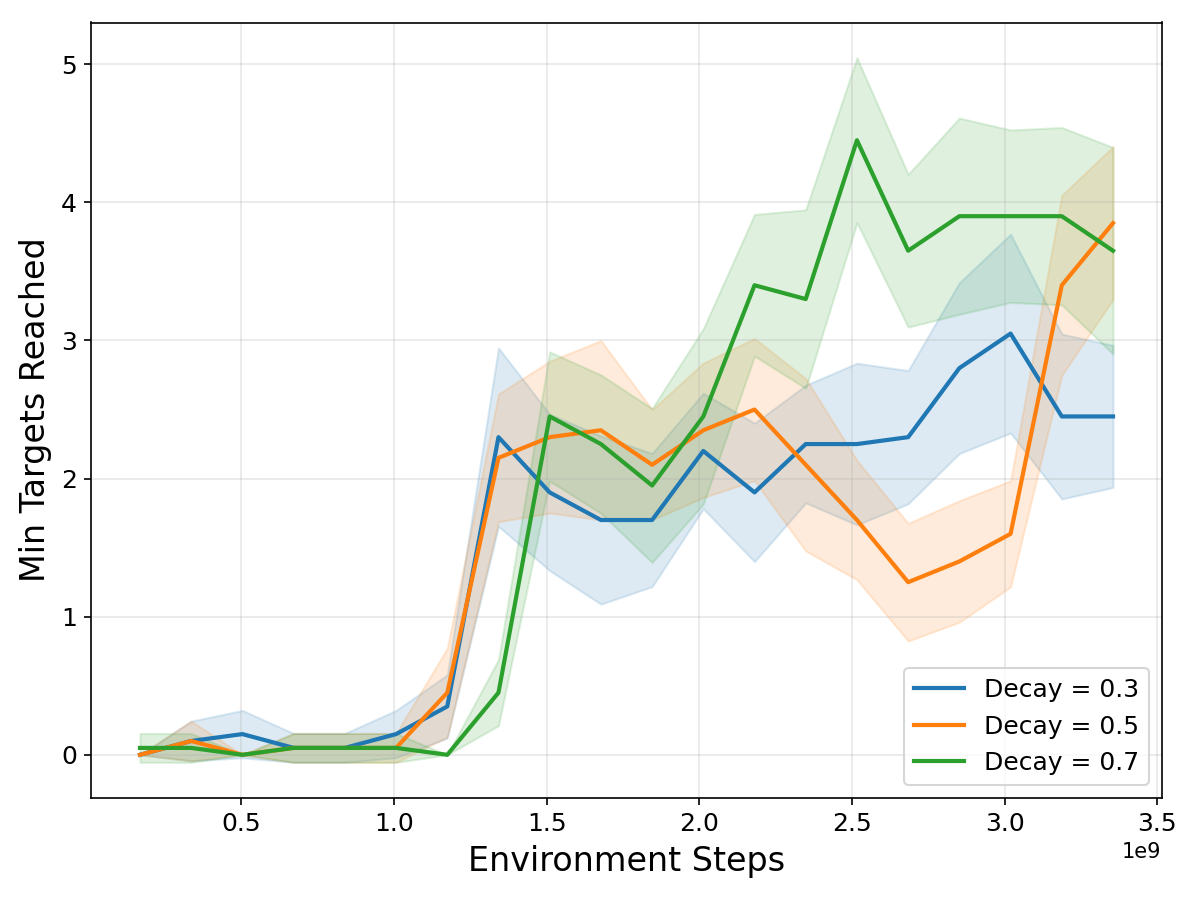
\includegraphics[width=0.5\textwidth]{img/gridworld_reward_decay_learning_curves.png}
    \caption{Reward decay. [Placeholder description.]}
    \label{fig:gridworld-reward-decay}
\end{figure}
